\documentclass[a4paper,12pt]{article}

\usepackage{tikz}
\usepackage{tabularx}
\usepackage{amsmath}
\usepackage[utf8]{inputenc}
\usepackage{multicol}
\usepackage{amsmath, amssymb, amsthm}
\usepackage{enumitem}
\usepackage{array}
\usepackage[left=2cm, right=2cm, top=2cm, bottom=2cm]{geometry}
\usepackage{fancyhdr}
\usepackage{xfp}
\usepackage{pgf}

\usepackage{graphicx}
\usepackage{fancyhdr}

\setlength{\headheight}{28pt}
\pagestyle{fancy}
\fancyhf{} % alles leeren

% Kopfzeile
\fancyhead[L]{\includegraphics[height=1.2cm]{logo.png}}
\fancyhead[C]{\small Beispielaufgaben-Klassenarbeit\\ Heinrich-von-Kleist-Schule}
\fancyhead[R]{\small Mathematik – G10B\\ Name:\ \rule{2.8cm}{0.4pt}}

% Fußzeile
\fancyfoot[C]{Seite \thepage \enspace\textbullet\enspace
	J.\,Mycan \textcopyright~2025\ *Klassenarbeit 45 min.*}

\renewcommand{\footrulewidth}{0.4pt}



\newcommand{\punkteA}{0}
\newcommand{\punkteB}{0}
\newcommand{\punkteC}{0}
\newcommand{\punkteD}{0}
\newcommand{\punkteE}{0}

\newcommand{\maxSumme}{45}
\newcommand{\noteEinsMin}{\fpeval{round(\maxSumme * 0.95,0)}}
\newcommand{\noteZweiMin}{\fpeval{round(\maxSumme * 0.80,0)}}
\newcommand{\noteDreiMin}{\fpeval{round(\maxSumme * 0.60,0)}}
\newcommand{\noteVierMin}{\fpeval{round(\maxSumme * 0.45,0)}}
\newcommand{\noteFunfMin}{\fpeval{round(\maxSumme * 0.20,0)}}
\newcommand{\noteSechsMin}{0}

\newcommand{\summe}{%
	\pgfmathparse{\punkteA + \punkteB + \punkteC + \punkteD + \punkteE}%
	\pgfmathprintnumber{\pgfmathresult}}

\begin{document}
%%%%%%%%%%%%%%%%%%%%%%%%%%%%%%%%%%%%%%%%%%%%%%%%%%%%
% LÖSUNGSTEIL
%%%%%%%%%%%%%%%%%%%%%%%%%%%%%%%%%%%%%%%%%%%%%%%%%%%%

\section*{Lösungen}

%%%%%%%%%%%%%%%%%%%%%%%%%%%%%%%%%%%%%%%%%%%%%%%%%%%%
% Lösung: Quadratische Gleichungen (Aufgabe 2)
%%%%%%%%%%%%%%%%%%%%%%%%%%%%%%%%%%%%%%%%%%%%%%%%%%%%

\subsection*{Lösung zu Aufgabe 2: Quadratische Gleichungen}

\begin{enumerate}
	
	\item[a)] \(\displaystyle 2x^2 - 5x + 1 = x^2 + 4x - 2\)
	
	\textbf{Schritt 1: Alle Terme auf eine Seite bringen.}
	\begin{align*}
		2x^2 - 5x + 1 &= x^2 + 4x - 2\\[2pt]
		2x^2 - 5x + 1 - x^2 - 4x + 2 &= 0\\[2pt]
		x^2 - 9x + 3 &= 0
	\end{align*}
	
	\textbf{Schritt 2: Mit der \emph{pq-Formel} lösen.}\\
	Wir schreiben
	\[
	x^2 - 9x + 3 = 0
	\]
	in der Form \(x^2 + px + q = 0\) mit \(p = -9,\; q = 3\).\\
	Die pq-Formel:
	\[
	x_{1,2} = -\frac{p}{2} \pm \sqrt{\left(\frac{p}{2}\right)^2 - q}
	\]
	
	\begin{align*}
		x_{1,2} 
		&= -\frac{-9}{2} \pm \sqrt{\left(\frac{-9}{2}\right)^2 - 3}\\[2pt]
		&= \frac{9}{2} \pm \sqrt{\frac{81}{4} - 3}\\[2pt]
		&= \frac{9}{2} \pm \sqrt{\frac{81}{4} - \frac{12}{4}}\\[2pt]
		&= \frac{9}{2} \pm \sqrt{\frac{69}{4}}\\[2pt]
		&= \frac{9}{2} \pm \frac{\sqrt{69}}{2}
	\end{align*}
	
	\[
	\boxed{x_1 = \frac{9 - \sqrt{69}}{2},\quad x_2 = \frac{9 + \sqrt{69}}{2}}
	\]
	
	% --------------------------------------------------
	
	\item[b)] \(\displaystyle (x - 3)^2 + 2x = 2x^2 - x + 5\)
	
	\textbf{Schritt 1: Klammer ausmultiplizieren.}
	\[
	(x-3)^2 = x^2 - 6x + 9
	\]
	
	Gleichung einsetzen:
	\begin{align*}
		x^2 - 6x + 9 + 2x &= 2x^2 - x + 5\\[2pt]
		x^2 - 4x + 9 &= 2x^2 - x + 5
	\end{align*}
	
	\textbf{Schritt 2: Alle Terme auf eine Seite.}
	\begin{align*}
		x^2 - 4x + 9 - 2x^2 + x - 5 &= 0\\[2pt]
		(-x^2) - 3x + 4 &= 0
	\end{align*}
	Wir multiplizieren mit \(-1\) (das ändert die Lösung nicht):
	\[
	x^2 + 3x - 4 = 0
	\]
	
	\textbf{Schritt 3: pq-Formel oder Faktorisieren.}
	
	Faktorisieren:
	\[
	x^2 + 3x - 4 = (x+4)(x-1)
	\]
	denn:
	\[
	(x+4)(x-1)=x^2 - x + 4x - 4 = x^2 + 3x - 4
	\]
	
	\[
	(x+4)(x-1) = 0 \quad\Rightarrow\quad
	\boxed{x_1 = -4,\; x_2 = 1}
	\]
	
	% --------------------------------------------------
	
	\item[c)] \(\displaystyle 3(x+1)^2 - 4 = 2x^2 + x + 5\)
	
	\textbf{Schritt 1: Klammer ausmultiplizieren.}
	\[
	(x+1)^2 = x^2 + 2x + 1
	\]
	daher:
	\[
	3(x+1)^2 = 3x^2 + 6x + 3
	\]
	
	Einsetzen:
	\begin{align*}
		3x^2 + 6x + 3 - 4 &= 2x^2 + x + 5\\[2pt]
		3x^2 + 6x - 1 &= 2x^2 + x + 5
	\end{align*}
	
	\textbf{Schritt 2: Alle Terme auf eine Seite.}
	\begin{align*}
		3x^2 + 6x - 1 - 2x^2 - x - 5 &= 0\\[2pt]
		x^2 + 5x - 6 &= 0
	\end{align*}
	
	\textbf{Schritt 3: Faktorisieren.}
	Wir suchen zwei Zahlen, deren Summe \(5\) und deren Produkt \(-6\) ist:
	\[
	6 \cdot (-1) = -6,\quad 6 + (-1) = 5
	\]
	Also:
	\[
	x^2 + 5x - 6 = (x+6)(x-1)
	\]
	\[
	(x+6)(x-1) = 0 \quad\Rightarrow\quad 
	\boxed{x_1 = -6,\; x_2 = 1}
	\]
	
	% --------------------------------------------------
	
	\item[d)] \(\displaystyle 2x(x-1) + 3 = (x-2)^2\)
	
	\textbf{Schritt 1: Klammern ausmultiplizieren.}
	\[
	2x(x-1) = 2x^2 - 2x
	\]
	\[
	(x-2)^2 = x^2 - 4x + 4
	\]
	
	Einsetzen:
	\begin{align*}
		2x^2 - 2x + 3 &= x^2 - 4x + 4
	\end{align*}
	
	\textbf{Schritt 2: Alle Terme auf eine Seite.}
	\begin{align*}
		2x^2 - 2x + 3 - x^2 + 4x - 4 &= 0\\[2pt]
		x^2 + 2x - 1 &= 0
	\end{align*}
	
	\textbf{Schritt 3: pq-Formel.}\\
	\(x^2 + 2x - 1 = 0 \Rightarrow p = 2,\; q = -1\)
	\[
	x_{1,2} = -\frac{p}{2} \pm \sqrt{\left(\frac{p}{2}\right)^2 - q}
	= -1 \pm \sqrt{1 - (-1)}
	= -1 \pm \sqrt{2}
	\]
	\[
	\boxed{x_1 = -1 + \sqrt{2},\quad x_2 = -1 - \sqrt{2}}
	\]
	
\end{enumerate}


%%%%%%%%%%%%%%%%%%%%%%%%%%%%%%%%%%%%%%%%%%%%%%%%%%%%
% Lösung: Potenzgleichungen (Aufgabe 4)
%%%%%%%%%%%%%%%%%%%%%%%%%%%%%%%%%%%%%%%%%%%%%%%%%%%%

%%%%%%%%%%%%%%%%%%%%%%%%%%%%%%%%%%%%%%%%%%%%%%%%%%%%
% LÖSUNG: Potenzgleichungen (Aufgabe 4)
%%%%%%%%%%%%%%%%%%%%%%%%%%%%%%%%%%%%%%%%%%%%%%%%%%%%

\subsection*{Lösung zu Aufgabe 4: Potenzgleichungen}

\begin{enumerate}
	\item[a)] $2^{x+1} + 8 = 4\cdot 2^{x}$
	
	\textbf{Schritt 1: Potenzregel nutzen.}
	\[
	2^{x+1} = 2\cdot 2^x
	\]
	Also:
	\[
	2\cdot 2^x + 8 = 4\cdot 2^x
	\]
	
	\textbf{Schritt 2: Alle Terme mit $2^x$ auf eine Seite bringen.}
	\begin{align*}
		2\cdot 2^x + 8 &= 4\cdot 2^x\\
		8 &= 4\cdot 2^x - 2\cdot 2^x\\
		8 &= 2\cdot 2^x
	\end{align*}
	
	\textbf{Schritt 3: Durch 2 teilen.}
	\[
	4 = 2^x
	\]
	
	\textbf{Schritt 4: 4 als Zweierpotenz schreiben.}
	\[
	4 = 2^2 \Rightarrow 2^x = 2^2 \Rightarrow x = 2
	\]
	
	\[
	\boxed{x = 2}
	\]
	
	%------------------------------------------------
	
	\item[b)] $5\cdot 3^{x} + 2 = 2\cdot 3^{x} + 29$
	
	\textbf{Schritt 1: Terme mit $3^x$ zusammenfassen.}
	\begin{align*}
		5\cdot 3^x + 2 &= 2\cdot 3^x + 29\\
		5\cdot 3^x - 2\cdot 3^x &= 29 - 2\\
		3\cdot 3^x &= 27
	\end{align*}
	
	\textbf{Schritt 2: Durch 3 teilen.}
	\[
	3^x = 9
	\]
	
	\textbf{Schritt 3: 9 als Dreierpotenz schreiben.}
	\[
	9 = 3^2 \Rightarrow 3^x = 3^2 \Rightarrow x = 2
	\]
	
	\[
	\boxed{x = 2}
	\]
	
	%------------------------------------------------
	
	\item[c)] $3^{2x} = 27\cdot 3^{x-1}$
	
	\textbf{Schritt 1: Rechte Seite zu einer Potenz vereinfachen.}
	\[
	27 = 3^3
	\]
	Also:
	\[
	27\cdot 3^{x-1} = 3^3\cdot 3^{x-1} = 3^{3 + x - 1} = 3^{x+2}
	\]
	
	Die Gleichung wird:
	\[
	3^{2x} = 3^{x+2}
	\]
	
	\textbf{Schritt 2: Exponenten vergleichen (Basis gleich und positiv).}
	\[
	2x = x + 2 \Rightarrow x = 2
	\]
	
	\[
	\boxed{x = 2}
	\]
	
	%------------------------------------------------
	
	\item[d)] $\left(\dfrac{1}{2}\right)^{x+1} = 4\cdot \left(\dfrac{1}{2}\right)^{2x}$
	
	\textbf{Schritt 1: $4$ als Potenz zur Basis $\tfrac{1}{2}$ schreiben.}
	\[
	4 = 2^2 = \left(\frac{1}{2}\right)^{-2}
	\]
	Dann:
	\[
	4\cdot \left(\frac{1}{2}\right)^{2x}
	= \left(\frac{1}{2}\right)^{-2}\cdot \left(\frac{1}{2}\right)^{2x}
	= \left(\frac{1}{2}\right)^{2x-2}
	\]
	
	Die Gleichung ist jetzt:
	\[
	\left(\frac{1}{2}\right)^{x+1} = \left(\frac{1}{2}\right)^{2x-2}
	\]
	
	\textbf{Schritt 2: Exponenten vergleichen.}
	\[
	x + 1 = 2x - 2 \Rightarrow x = 3
	\]
	
	\[
	\boxed{x = 3}
	\]
	
\end{enumerate}


%%%%%%%%%%%%%%%%%%%%%%%%%%%%%%%%%%%%%%%%%%%%%%%%%%%%
% Lösung: Abstand Punkt – Gerade (Aufgabe ?)
%%%%%%%%%%%%%%%%%%%%%%%%%%%%%%%%%%%%%%%%%%%%%%%%%%%%

\subsection*{Lösung: Punkt mit minimalem Abstand zur Geraden}

Gegeben:
\[
g:\; y = x + 1,\quad Q(3\mid -1)
\]

Gesucht: Punkt \(P\) auf \(g\) mit minimalem Abstand zu \(Q\) und dieser minimale Abstand.

\paragraph{Idee:} Der kürzeste Abstand von einem Punkt zu einer Geraden ist immer entlang der Senkrechten zur Geraden. Also suchen wir die Gerade \(h\), die durch \(Q\) geht und \emph{senkrecht} zu \(g\) ist. Dann ist \(P\) der Schnittpunkt von \(g\) und \(h\).

\subsubsection*{1. Schritt: Steigung der Senkrechten}

Gerade \(g\) hat Steigung \(m_g = 1\).  
Eine senkrechte Gerade hat Steigung
\[
m_h = -\frac{1}{m_g} = -1.
\]

Gerade \(h\) hat also die Form:
\[
h:\; y = -x + b.
\]

\subsubsection*{2. Schritt: Gerade \(h\) durch \(Q(3\mid -1)\)}

Punkt \(Q\) liegt auf \(h\), also muss gelten:
\[
y_Q = -x_Q + b
\]
Einsetzen von \(Q(3\mid -1)\):
\[
-1 = -3 + b \Rightarrow b = 2.
\]

Damit:
\[
h:\; y = -x + 2.
\]

\subsubsection*{3. Schritt: Schnittpunkt \(P\) von \(g\) und \(h\)}

Schnittpunkt \(P\) liegt auf beiden Geraden, also:
\[
x + 1 = -x + 2
\]

\textbf{Gleichung lösen:}
\begin{align*}
	x + 1 &= -x + 2\\[2pt]
	x + x &= 2 - 1\\[2pt]
	2x &= 1\\[2pt]
	x &= \frac{1}{2}
\end{align*}

\[
y = x + 1 = \frac{1}{2} + 1 = \frac{3}{2}
\]

\[
\boxed{P\left(\frac{1}{2}\;\middle|\; \frac{3}{2}\right)}
\]

\subsubsection*{4. Schritt: Minimaler Abstand \(|PQ|\)}

Abstand zweier Punkte \(P(x_P,y_P)\) und \(Q(x_Q,y_Q)\):
\[
d(P,Q) = \sqrt{(x_Q - x_P)^2 + (y_Q - y_P)^2}
\]

Einsetzen:
\[
x_P = \frac{1}{2},\; y_P = \frac{3}{2},\quad
x_Q = 3,\; y_Q = -1
\]

\begin{align*}
	d &= \sqrt{\left(3 - \frac{1}{2}\right)^2 + \left(-1 - \frac{3}{2}\right)^2}\\[2pt]
	&= \sqrt{\left(\frac{5}{2}\right)^2 + \left(-\frac{5}{2}\right)^2}\\[2pt]
	&= \sqrt{\frac{25}{4} + \frac{25}{4}}\\[2pt]
	&= \sqrt{\frac{50}{4}}\\[2pt]
	&= \sqrt{\frac{25}{2}}\\[2pt]
	&= \frac{5}{\sqrt{2}} = \frac{5\sqrt{2}}{2}
\end{align*}

\[
\boxed{d_{\min} = \frac{5\sqrt{2}}{2} \approx 3{,}54}
\]

\subsubsection*{5. Schritt: Skizze (TikZ)}

\begin{center}
	\begin{tikzpicture}[scale=0.8]
		% Gitter
		\draw[step=1,very thin,gray!40] (-1,-3) grid (5,3);
		% Achsen
		\draw[->] (-1,0) -- (5.3,0) node[right] {$x$};
		\draw[->] (0,-3) -- (0,3.3) node[above] {$y$};
		
		% Gerade g: y = x + 1
		\draw[thick] (-1,0) -- (4,5); % verlängert, nur Ausschnitt sichtbar
		
		% Gerade h: y = -x + 2
		\draw[thick,dashed] (-1,3) -- (4,-2);
		
		% Punkte Q und P
		\fill (3,-1) circle (2pt) node[below right] {$Q(3\mid -1)$};
		\fill (0.5,1.5) circle (2pt) node[above left] {$P\!\left(\tfrac{1}{2}\mid\tfrac{3}{2}\right)$};
		
		% Senkrechte Verbindung
		\draw[very thick] (3,-1) -- (0.5,1.5);
	\end{tikzpicture}
\end{center}


%%%%%%%%%%%%%%%%%%%%%%%%%%%%%%%%%%%%%%%%%%%%%%%%%%%%
% Lösung: Rechteck im Dreieck (Extremwert)
%%%%%%%%%%%%%%%%%%%%%%%%%%%%%%%%%%%%%%%%%%%%%%%%%%%%

\subsection*{Lösung: Rechteck im Dreieck (Extremwertaufgabe)}

Wir verwenden das Dreieck aus deiner Aufgabe (z.\,B. mit den Eckpunkten)
\[
A(-2\mid 0),\; B(6\mid 0),\; C(0\mid 4).
\]

Das Rechteck liegt mit der unteren Seite auf der \(x\)-Achse, die beiden oberen Ecken
liegen auf den beiden Schenkeln \(\overline{AC}\) und \(\overline{BC}\).

\subsubsection*{1. Schritt: Geradengleichungen der Schenkel}

Gerade durch \(A(-2,0)\) und \(C(0,4)\):
\[
m_{AC} = \frac{4-0}{0-(-2)} = \frac{4}{2} = 2.
\]
Ansatz \(y = 2x + b\). Einsetzen von \(A(-2,0)\):
\[
0 = 2\cdot(-2) + b \Rightarrow 0 = -4 + b \Rightarrow b = 4.
\]
\[
AC:\; y = 2x + 4
\]

Gerade durch \(B(6,0)\) und \(C(0,4)\):
\[
m_{BC} = \frac{0-4}{6-0} = \frac{-4}{6} = -\frac{2}{3}.
\]
Ansatz \(y = -\tfrac{2}{3}x + b\). Einsetzen von \(B(6,0)\):
\[
0 = -\tfrac{2}{3}\cdot 6 + b = -4 + b \Rightarrow b = 4.
\]
\[
BC:\; y = -\tfrac{2}{3}x + 4
\]

\subsubsection*{2. Schritt: Rechteckhöhe als Variable \(y\)}

Sei \(y > 0\) die Höhe des Rechtecks.  
Dann schneiden die Horizontalen \(y = \text{konstant}\) die Schenkel in den Punkten:

\begin{itemize}
	\item Links auf \(AC:\; y = 2x + 4 \Rightarrow x_\text{links} = \dfrac{y-4}{2}\)
	\item Rechts auf \(BC:\; y = -\tfrac{2}{3}x + 4 \Rightarrow 
	-\tfrac{2}{3}x = y-4 \Rightarrow x_\text{rechts} = \tfrac{3}{2}(4-y)\)
\end{itemize}

\subsubsection*{3. Schritt: Breite und Flächeninhalt des Rechtecks}

Breite:
\begin{align*}
	b(y) &= x_\text{rechts} - x_\text{links}\\[2pt]
	&= \tfrac{3}{2}(4-y) - \frac{y-4}{2}\\[2pt]
	&= \frac{3(4-y) - (y-4)}{2}\\[2pt]
	&= \frac{12 - 3y - y + 4}{2}\\[2pt]
	&= \frac{16 - 4y}{2}\\[2pt]
	&= 8 - 2y
\end{align*}

Flächeninhalt:
\[
A(y) = \text{Breite} \cdot \text{Höhe} = b(y)\cdot y = (8 - 2y)\cdot y = 8y - 2y^2
\]

Das ist eine nach unten geöffnete Parabel.

\subsubsection*{4. Schritt: Maximum des Flächeninhalts}

Parabel \(A(y) = -2y^2 + 8y\).  
Scheitelpunkt liegt bei
\[
y_S = -\frac{b}{2a} = -\frac{8}{2\cdot(-2)} = -\frac{8}{-4} = 2.
\]

Maximale Höhe:
\[
y_{\max} = 2.
\]

Breite bei \(y = 2\):
\[
b(2) = 8 - 2\cdot 2 = 8 - 4 = 4.
\]

Maximaler Flächeninhalt:
\[
A_{\max} = A(2) = 8\cdot 2 - 2\cdot 2^2 = 16 - 8 = 8.
\]

\[
\boxed{A_{\max} = 8\ \text{Flächeneinheiten}}
\]

Koordinaten der Eckpunkte des optimalen Rechtecks:
\[
x_\text{links} = \frac{2-4}{2} = -1,\quad
x_\text{rechts} = \tfrac{3}{2}(4-2) = \tfrac{3}{2}\cdot 2 = 3.
\]
Eckpunkte:
\[
(-1,0),\; (3,0),\; (3,2),\; (-1,2).
\]

\subsubsection*{5. Schritt: Skizze}

\begin{center}
	\begin{tikzpicture}[scale=0.7]
		% Gitter
		\draw[step=1,very thin,gray!40] (-3,-1) grid (7,5);
		% Achsen
		\draw[->] (-3,0) -- (7.3,0) node[right] {$x$};
		\draw[->] (0,-1) -- (0,5.3) node[above] {$y$};
		
		% Dreieck
		\coordinate (A) at (-2,0);
		\coordinate (B) at (6,0);
		\coordinate (C) at (0,4);
		\draw[thick] (A) -- (C) -- (B) -- cycle;
		
		% Optimales Rechteck
		\coordinate (R1) at (-1,0);
		\coordinate (R2) at (3,0);
		\coordinate (R3) at (3,2);
		\coordinate (R4) at (-1,2);
		
		\fill[green!30] (R1) -- (R2) -- (R3) -- (R4) -- cycle;
		\draw[thick] (R1) -- (R2) -- (R3) -- (R4) -- cycle;
		
		% Beschriftung
		\node[below] at (A) {$A(-2\mid 0)$};
		\node[below] at (B) {$B(6\mid 0)$};
		\node[above] at (C) {$C(0\mid 4)$};
		
		\node[below] at (R1) {$(-1\mid 0)$};
		\node[below] at (R2) {$(3\mid 0)$};
		\node[right] at (R3) {$(3\mid 2)$};
		\node[left]  at (R4) {$(-1\mid 2)$};
	\end{tikzpicture}
\end{center}


%%%%%%%%%%%%%%%%%%%%%%%%%%%%%%%%%%%%%%%%%%%%%%%%%%%%
% Lösung: Zuordnung Potenzfunktionen (Aufgabe 6)
%%%%%%%%%%%%%%%%%%%%%%%%%%%%%%%%%%%%%%%%%%%%%%%%%%%%

\subsection*{Lösung zu Aufgabe 6: Zuordnung Potenzfunktionen}

(Es werden die Graphen 1–8 aus der Aufgabenstellung vorausgesetzt.)

\begin{itemize}
	\item Graph \textbf{1}: nach oben geöffnete Parabel, symmetrisch zur \(y\)-Achse,
	wächst für \(|x|\) groß schnell nach oben  
	\(\Rightarrow f(x) = x^2\) (bei dir: Antwort A)
	\item Graph \textbf{2}: S-förmiger Verlauf durch Ursprung, ungerade Funktion,
	fällt für \(x<0\), steigt für \(x>0\)  
	\(\Rightarrow f(x) = x^3\) (Antwort A)
	\item Graph \textbf{3}: nur für \(x\ge 0\), startet im Ursprung,
	flacht nach rechts stark ab  
	\(\Rightarrow f(x) = \sqrt{x}\) (Antwort A)
	\item Graph \textbf{4}: Spiegelung von \(\sqrt{x}\) an der \(x\)-Achse,
	nur für \(x\ge 0\)  
	\(\Rightarrow f(x) = -\sqrt{x}\) (Antwort A)
	\item Graph \textbf{5}: Hyperbel mit zwei Ästen in Quadranten I und III,
	geht nie durch den Ursprung, senkrechte und waagrechte Asymptote  
	\(\Rightarrow f(x) = \dfrac{1}{x}\) (Antwort A)
	\item Graph \textbf{6}: Hyperbel mit beiden Ästen über der \(x\)-Achse
	(Quadranten I und II), symmetrisch zur \(y\)-Achse  
	\(\Rightarrow f(x) = \dfrac{1}{x^2}\) (Antwort A)
	\item Graph \textbf{7}: nur für \(x>0\), stark abfallend, nähert sich der
	\(x\)-Achse, geht aber nach oben gegen \(\infty\), wenn \(x\to 0^+\)  
	\(\Rightarrow f(x) = \dfrac{1}{\sqrt{x}}\) (Antwort A)
	\item Graph \textbf{8}: kubikwurzelähnlicher Verlauf, geht durch den Ursprung,
	flach für große \(|x|\), definiert für alle \(x\), aber weniger steil als \(x^3\)  
	\(\Rightarrow f(x) = x^{1/3}\) (Antwort A)
\end{itemize}

\bigskip
% Ende Lösungsteil

	
\end{document}
